\documentclass[semifinal]{cpecmu}

%% This is a sample document demonstrating how to use the CPECMU
%% project template. If you are having trouble, see "cpecmu.pdf" for
%% documentation.


%%%%% Init Commands
%
%
\englishtrue
%
%
%%%%%

\projectNo{S003-1/66}
\acadyear{2023}

\titleTH{ปัญญาประดิษฐ์สำหรับเกมกระดานรูท}
\titleEN{Artificial Intelligence for Root Board Game}

\author{นายบางกอก วาณิชยานนท์}{Baangkok Vanijyananda}{630610746}
\author{นายปวเรศ ดิลกวุฒิสิทธิ์}{Pawaret Dilokwuttisit}{630610748}

\cpeadvisor{kasemsit}
\cpecommittee{karn}
\cpecommittee{navadon}
% \committee{รศ.ดร.\,นิพนธ์ ธีรอำพน}{Assoc.\,Prof.\,Nipon Theera-Umpon, Ph.D.}

%% Some possible packages to include:
\usepackage[final]{graphicx} % for including graphics

%% Add bookmarks and hyperlinks in the document.
\PassOptionsToPackage{hyphens}{url}
\usepackage[colorlinks=true,allcolors=Blue4,citecolor=red,linktoc=all]{hyperref}
\def\UrlLeft#1\UrlRight{$#1$}

%% Needed just by this example, but maybe not by most reports
\usepackage{afterpage} % for outputting
\usepackage{pdflscape} % for landscape figures and tables. 

%% Some other useful packages. Look these up to find out how to use
%% them.
% \usepackage{natbib}    % for author-year citation styles
% \usepackage{txfonts}
% \usepackage{appendix}  % for appendices on a per-chapter basis
% \usepackage{xtab}      % for tables that go over multiple pages
% \usepackage{subfigure} % for subfigures within a figure
% \usepackage{pstricks,pdftricks} % for access to special PostScript and PDF commands
% \usepackage{nomencl}   % if you have a list of abbreviations

%% if you're having problems with overfull boxes, you may need to increase
%% the tolerance to 9999
% \tolerance=9999

\bibliographystyle{plain}
% \bibliographystyle{IEEEbib}

% \renewcommand{\topfraction}{0.85}
% \renewcommand{\textfraction}{0.1}
% \renewcommand{\floatpagefraction}{0.75}

%% Example for glossary entry
%% Need to use glossary option
%% See glossaries package for complete documentation.
\ifglossary
  \newglossaryentry{lorem ipsum}{
    name=lorem ipsum,
    description={derived from Latin dolorem ipsum, translated as ``pain itself''}
  }
\fi

%% Uncomment this command to preview only specified LaTeX file(s)
%% imported with \include command below.
%% Any other file imported via \include but not specified here will not
%% be previewed.
%% Useful if your report is large, as you might not want to build
%% the entire file when editing a certain part of your report.
% \includeonly{chapters/intro,chapters/background}

\begin{document}
\newcommand{\Marquise}{Marquise de Cat}
\newcommand{\Eyrie}{Eyrie Dynasties}
\newcommand{\RootB}{Root board game}
\newcommand{\RootV}{Root video game}
\newcommand{\RootOurs}{RootMinimal}
\newcommand{\RootAI}{RootTrainer}
\newcommand{\tabitem}{~~{\textbullet}~~}
\newcommand{\tabsubitem}{~~{\quad \textbullet}~~}


\maketitle
\makesignature

\ifproject
\begin{abstractTH}
เป้าหมายของโครงการนี้คือ การพัฒนาระบบปัญญาประดิษฐ์ที่สามารถเล่นเกมกระดาน ``Root'' ได้อย่างชาญฉลาดและมีประสิทธิภาพ โดยระบบจะรับ state ปัจจุบันของเกม และทำการตัดสินใจเลือกทำ action ต่างๆในระหว่างการเล่น

Root เป็นเกมอสมมาตรที่สามารถสังเกตได้บางส่วน โดยผู้เล่นแต่ละคนมีกลไกเกมและเป้าหมายที่แตกต่างกัน เกมกระดาน Root ประกอบไปด้วยหลายเผ่า แต่ละเผ่ามีวิธีไปถึงการชนะได้แตกต่างกัน ในโครงการนี้เราจะสนใจที่ 2 เผ่าหลัก ได้แก่เผ่า ``Marquise'' de Cat และเผ่า the ``Eyrie'' Dynasties

อัลกอริทึมหลักที่เราจะใช้ในการสร้างปัญญาประดิษฐ์คือ Monte Carlo Tree Search (MCTS) ซึ่งจะหาความน่าจะเป็นในการชนะของแต่ละ action ที่ทำได้โดยการลองเล่นด้วย action นั้นหลายๆรอบ จากนั้นเลือก action ที่ทำให้ความน่าจะเป็นในการชนะสูงที่สุด

อัลกอริทึม MCTS มี parameters หลายตัว นั่นทำให้มี variant ของ MCTS อยู่หลาย variant เราจะนำ MCTS แต่ละ variant มาแข่งเพื่อหา variant ของ MCTS ที่ดีที่สุดสำหรับแต่ละเผ่า

% เขียนบทคัดย่อของโครงงานที่นี่

% การเขียนรายงานเป็นส่วนหนึ่งของการทำโครงงานวิศวกรรมคอมพิวเตอร์
% เพื่อทบทวนทฤษฎีที่เกี่ยวข้อง อธิบายขั้นตอนวิธีแก้ปัญหาเชิงวิศวกรรม และวิเคราะห์และสรุปผลการทดลองอุปกรณ์และระบบต่างๆ
% \enskip อย่างไรก็ดี การสร้างรูปเล่มรายงานให้ถูกรูปแบบนั้นเป็นขั้นตอนที่ยุ่งยาก
% แม้ว่าจะมีต้นแบบสำหรับใช้ในโปรแกรม Microsoft Word แล้วก็ตาม
% แต่นักศึกษาส่วนใหญ่ยังคงค้นพบว่าการใช้งานมีความซับซ้อน และเกิดความผิดพลาดในการจัดรูปแบบ กำหนดเลขหัวข้อ และสร้างสารบัญอยู่
% \enskip ภาควิชาวิศวกรรมคอมพิวเตอร์จึงได้จัดทำต้นแบบรูปเล่มรายงานโดยใช้ระบบจัดเตรียมเอกสาร
% \LaTeX{} เพื่อช่วยให้นักศึกษาเขียนรายงานได้อย่างสะดวกและรวดเร็วมากยิ่งขึ้น
\end{abstractTH}

\begin{abstract}
Our goal is to develop an artificial intelligence (AI) system capable of playing the board game ``Root''. Our objective is to create an intelligent agent that can take game state as input and make intelligent decisions in each phase.


Root is a partially observable asymmetric game where each player has different game mechanics and goals. There are many factions within Root, each having its own way to achieve victory conditions. We will focus on two base factions: ``Marquise'' de Cat and the ``Eyrie'' Dynasties.

Our main algorithm for implementing the AI is Monte Carlo Tree Search (MCTS). MCTS algorithm maximizes the probability of winning by simulating many rollouts and choosing the best decision.

There are multiple parameters for the MCTS algorithm resulting in multiple variants of MCTS algorithms. We will pitch different variants of MCTS together with aim to find the best MCTS variant for each faction.

% To build the AI, we will construct multiple AI agents and have them play against one another so they can both improve themselves. Each agent will have different versions built from different algorithms, including Monte Carlo Tree Search, Neural Network Reinforcement Learning, random, weighted-random, hard-coded, human player, etc.

% We aim to develop an artificial intelligence (AI) system capable of playing the board game "Root." Our objective is to create an intelligent agent that can take game state as input, make decisions in each phase, and compete against the AI in the digital adaptation video game of the board game Root.

% Root is a partially observable asymmetric game where each player has different game mechanics and goals. This can be applied to real-world problems where different parties have different goals but are in the same area, so they have to compete to take hold of the limited resources needed to complete their goals.

% To build the AI, we will have an agent play against another agent so they can both learn. Each agent will have different versions built from different algorithms, including Monte Carlo Tree Search, Neural Network Reinforcement Learning, random, weighted-random, hard-coded, human player, etc.
% ------
% The abstract would be placed here. It usually does not exceed 350 words
% long (not counting the heading), and must not take up more than one (1) page
% (even if fewer than 350 words long).

% Make sure your abstract sits inside the \texttt{abstract} environment.
\end{abstract}

\iffalse
\begin{dedication}
This document is dedicated to all Chiang Mai University students.

Dedication page is optional.
\end{dedication}
\fi % \iffalse

\begin{acknowledgments}
We would like to express my deep appreciation for Asst. Prof. Kasemsit Teeyapan, Ph.D. for his exceptional dedication, expertise, and detailed guidance throughout the project, which served as a constant source of inspiration and helped ensure its successful completion.
% Your acknowledgments go here. Make sure it sits inside the
% \texttt{acknowledgment} environment.

\acksign{2024}{02}{18}
\end{acknowledgments}%
\fi % \ifproject

\contentspage

\ifproject
\figurelistpage

\tablelistpage
\fi % \ifproject

% \abbrlist % this page is optional

% \symlist % this page is optional

% \preface % this section is optional


\pagestyle{empty}\cleardoublepage
\normalspacing \setcounter{page}{1} \pagenumbering{arabic} \pagestyle{cpecmu}

\chapter{\ifenglish Introduction\else บทนำ\fi}

\section{\ifenglish Project rationale\else ที่มาของโครงงาน\fi}
Artificial intelligence (AI) has revolutionized the world of video games by giving players friends to play with or foes to play against. The digital adaptation video game of the \RootB{} is no exception. But there are problems with the AIs. There are multiple reports by \RootV{} players that the AIs are no longer challenging to play against once you start to know how to play your faction or that the AIs make awful decisions that no humans would ever make in a similar situation.

This project focuses on the recommended scenario in a two-player game of \Marquise{} faction versus \Eyrie{} faction since they are both empire factions, i.e., factions with many buildings and warriors on the board, thus making this scenario have a lot of interactions.

%%%%%
%
% Maybe we should move this paragraph vvv to background chapter 
%
\Marquise{} requires players to balance building types to be able to continuously grow and earn points, while \Eyrie{} requires players to carefully build and follow \textit{the Decree}, which can get very powerful, but failing to follow it will result in a setback in the form of losing points. The relevant rules of Root will be explained in this document.
%
%%%%%

This project aims to create an artificial intelligence (AI) system capable of playing the board game ``Root'' that is more intelligent than the AIs in the \RootV{}. The agents will be built using different methods, including Monte Carlo tree search, neural network reinforcement learning, random, human player, etc. Full details on each AI agent implementation method and their concepts are explained in this document.

% Root features a variety of factions, each with its unique gameplay mechanics and goals. 

% We will implement our own version of Root video game in Python which allows us to freely control the environment and integrate with other libraries for developing game AIs. Then  

% Our objective is to create an intelligent agent that can take game state as input, make decisions in each phase, and compete against the AI in the digital adaptation video game of the board game Root.

% One of these factions, the Eyrie Dynasties, presents a particularly intricate challenge when it comes to AI gameplay due to its unique mechanics that allows it to lose victory points. This project aims to address the existing limitations in AI within the Root video game, focusing on enhancing the experience for the Eyrie Dynasties faction.


\section{\ifenglish Objectives\else วัตถุประสงค์ของโครงงาน\fi}
\begin{itemize}
    \item To create an artificial intelligence (AI) that can play the board game ``Root'' and win against the AIs in the \RootV{}.
    % \item To create a version of Root video game with integrated AI agent training lifecycle which also allows human players to play against the AI agents.
\end{itemize}

\section{\ifenglish Project scope\else ขอบเขตของโครงงาน\fi}
% TODO: should i use AI agent training wrapper? training framework? training lifecycle?
The project is a software consisting of two main components: 1.) \textit{\RootOurs{}}, a minimal version of \RootV{}. 2.) \textit{\RootAI{}}, an AI agent training framework for \RootOurs{}. The scope of the project are as follows:
\begin{enumerate}
    \item Implementation of \RootOurs{}.
    \item Implementation of \RootAI{}.
    \item Exclude direct integration with \RootV{}, i.e., no pulling data from a running \RootV{}, and no injecting decisions into a running \RootV{} via code.
    \item Exclude direct integration with \RootB{}, i.e., no computer vision will be used to detect the state of the board game.
\end{enumerate}

\RootOurs{} supports the rules of Root [\ref{brief-rules-of-root}] in the scenario of \Marquise{} versus \Eyrie{}. Game mechanics not used by these two factions are not included. The scope of \RootOurs{} are as follows:
\begin{enumerate}
    \item Only \Marquise{} and \Eyrie{} factions.
    \item Only ``Woodland'' map.
    \item Exclude \textit{forests} area.
    \item Exclude building type \textit{ruins}.
    % \item \Marquise{} starts with their \textit{the Keep} token in the bottom right \textit{clearing}.
    % \item \Marquise{} starts with their three starting buildings pre-placed.
    % \item \Eyrie{} starts with a \textit{roost} in the top left clearing.
    % \item \Eyrie{} starts with the \textit{charismatic} leader.
\end{enumerate}

\RootAI{} has the following features:
\begin{enumerate}
    \item Importing and exporting of \RootOurs{}'s game state.
    \item Exporting of \RootOurs{}'s log.
    \item Interface for human interaction to an instance of \RootOurs{}.
    \item Training and running AI agents built using the following methods:
    \begin{itemize}
        \item Random decision
        \item Monte Carlo tree search (MCTS)
        \item Reinforcement learning neural network
    \end{itemize}
\end{enumerate}

% \subsection{\ifenglish Hardware scope\else ขอบเขตด้านฮาร์ดแวร์\fi}

% \subsection{\ifenglish Software scope\else ขอบเขตด้านซอฟต์แวร์\fi}

\section{\ifenglish Expected outcomes\else ประโยชน์ที่ได้รับ\fi}
\begin{itemize}
    \item The resulting AIs are able to win against \RootV{}'s corresponding opponent faction AI, i.e.:
    \begin{itemize}
        \item Resulting \Marquise{} AI have higher win rate against \RootV{}'s \Eyrie{} AI.
        \item Resulting \Eyrie{} AI have higher win rate against \RootV{}'s \Marquise{} AI.
    \item Root players have a more challenging opponent when playing by themselves.
    \end{itemize}
\end{itemize}

\section{\ifenglish Technology and tools\else เทคโนโลยีและเครื่องมือที่ใช้\fi}
Python is chosen as the language for this project's implementation due to its flexibility of integrating with AI related libraries such as PyTorch and Tensorflow. 

% \subsection{\ifenglish Hardware technology\else เทคโนโลยีด้านฮาร์ดแวร์\fi}
% \textit{Maybe add the gpu use and cloud use in the future}

\subsection{\ifenglish Software technology\else เทคโนโลยีด้านซอฟต์แวร์\fi}
%% TODO: add citations to each item's docs
% there are more
\textbf{Programming Languages:}
\begin{itemize}
    \item Python
\end{itemize}
% there are more
\textbf{Important Libraries:}
\begin{itemize}
    \item Pygame (UI) 
    \item PyTorch (RLNN)
    \item TensorFlow (RLNN)
\end{itemize}

\section{\ifenglish Project plan\else แผนการดำเนินงาน\fi}

\begin{plan}{6}{2023}{3}{2024}
    \planitem{6}{2023}{1}{2024}{\RootOurs \ implementation}
    \planitem{11}{2023}{3}{2024}{\RootAI \ implementation}
    \planitem{10}{2023}{11}{2023}{Agent:\textbf{Random}: Implementation}
    \planitem{10}{2023}{11}{2023}{Agent:\textbf{Random}: Simulation}
    \planitem{10}{2023}{11}{2023}{Agent:\textbf{Random}: Analysis and Documentation}
    \planitem{11}{2023}{1}{2024}{Agent:\textbf{MCTS}: Implementation}
    \planitem{12}{2023}{1}{2024}{Agent:\textbf{MCTS}: Simulation}
    \planitem{1}{2024}{1}{2024}{Agent:\textbf{MCTS}: Analysis and Documentation}
    \planitem{1}{2024}{3}{2024}{Agent:\textbf{RLNN}: Implementation}
    \planitem{2}{2024}{3}{2024}{Agent:\textbf{RLNN}: Simulation}
    \planitem{3}{2024}{3}{2024}{Agent:\textbf{RLNN}: Analysis and Documentation}
    \planitem{3}{2024}{3}{2024}{Document Finalization}
\end{plan}

\section{\ifenglish Roles and responsibilities\else บทบาทและความรับผิดชอบ\fi}
In \RootOurs{}, base classes and faction-neutral functions are divided equally among the two of us. Pawaret is responsible for \Marquise{}-related functionalities. Baangkok is responsible for \Eyrie{}-related functionalities.

In \RootAI{}, each step is divided equally, starting from method research to implementation to testing. This allows us to continuously exchange our knowledge about the current AI agent implementation method, allowing us to create and improve each AI agent to have good performance.

\section{\ifenglish%
Impacts of this project on society, health, safety, legal, and cultural issues
\else%
ผลกระทบด้านสังคม สุขภาพ ความปลอดภัย กฎหมาย และวัฒนธรรม
\fi}
This project can work as a foundation for future research on reinforcement learning, asymmetrical games, game AI, and other related topics.

\chapter{\ifenglish Background Knowledge and Theory\else ทฤษฎีที่เกี่ยวข้อง\fi}

In order to create the AI, we first need to implement \RootOurs{}. This requires knowledge of game programming fundamentals and extensive knowledge of the rules of \RootB{}. However, there are minor rule differences between \RootV{} and \RootB{}. Since \RootV{}`s AIs are the root cause of our project, we also need to find and implement these minor differences in our \RootOurs{}.

The next step is to implement \RootAI{}, the framework for running \RootOurs{} and training AI agents. There are two AI agent implementation methods that require additional self-study: Monte Carlo tree search and reinforcement learning neural networks.

\section{Root}
Root is an \textbf{asymetric game}: a game where each player starts with different setups, gameplay mechanics, etc. \cite{Mike_Shor-2023-10-06}. Although Root's base actions, such as move and battle, are the same for every faction, each faction starts differently, and each has its own unique mechanics and rules. Thus, Root sits closer to the asymmetric side in the symmetric-asymmetric spectrum. \\
Examples of symmetric games are Chess, Monopoly, Prisoner's Dilemma, etc.\\
Examples of other asymmetric games are Tapestry, Dune, Cthulhu Wars, etc.

Root is an \textbf{imperfect information game}: a game where there is information hidden from the player \cite{osborne1994course}. Most elements of Root, such as warrior placement, building count, etc., are laid out for all players to see. But cards on the player's hand are only visible to that player, i.e., other players' cards in hand are the hidden information in this game.

Root is a \textbf{non-deterministic game}: a game where there is some element of randomness involved, such as rolling dice or shuffling cards. Root has both, rolling dice in battle and drawing cards from a shuffled draw pile.

\subsection{Brief Rules of Root} \label{brief-rules-of-root}

Root is a turn-based game for 2-4 players in which you fight as one of four factions against other factions to take control of the ``Woodland''.

The rule is simple: The player who scores 30 victory points or plays the dominance card and fulfills its condition (the card that changes the endgame win condition) first wins. The players play on the map of Woodland (Figure \ref{fig:root-game-board}), which contains 12 clearings, each with different suits and a different number of slots for building. There are also paths that connect those clearings, moving warriors from one clearing to another.

\begin{figure}
  \begin{center}
    \includegraphics[width=\textwidth]{root_game_board.jpg}
  \end{center}
  \caption{Woodland, Root's game board}
  \label{fig:root-game-board}
\end{figure}

Each player will take his turn throughout three phases: birdsong, daylight, and evening. The player will be instructed on what he must do and what actions he can take in each phase. Also, each faction will have special abilities that can be used during their turn. Instructions and actions will vary from faction to faction, but there are actions that are shared by all factions, called key actions. There are three key actions:

\begin{enumerate}
  \item \textbf{Move}: Take any number of your warriors from one clearing and move them to one adjacent clearing.
  \item \textbf{Craft}: Using crafting pieces you have to craft a card from your hand. After crafting, gain benefits or effects on the crafted card.
  \item \textbf{Battle}: Choose a clearing where you have warriors as the clearing of battle. You are the attacker. Choose another player in the clearing of battle to be the defender. Roll two dice. The attacker deals hits equal to the higher roll, and the defender deals hits equal to the lower roll. Both players deal hits simultaneously and remove pieces equal to the number of hits they receive.
\end{enumerate}

Other than key actions, there will be some specific actions belonging to each faction. We will describe them in detail with an explanation of how each phase of each faction works in Tables \ref{tab:marquise-flow} and \ref{tab:eyrie-flow}.

Some of the rules will not be explained here, as they are not crucial or essential. For more details on rules, see \cite{RootBoardGameRules}.

\renewcommand{\arraystretch}{1.5}

% \afterpage{
  % \begin{landscape}
\begin{table}
  \caption{\Marquise{} Flow}
  \label{tab:marquise-flow}
  \centering
  \resizebox{\textwidth}{!}{\begin{tabular}{|p{3cm}|p{9cm}|p{4cm}|} 
    \hline
    \multicolumn{3}{|c|}{\Marquise} \\
    \hline
    Birdsong & Daylight & Evening \\ 
    \hline
    \tabitem Place one wood token at each sawmill. 
  & \tabitem Craft any cards in your hand using workshops.

    \tabitem Take up to three of the following actions (plus one per bird suit card you spend): 
    
      \tabsubitem Battle

      \tabsubitem March: Takes two moves

      \tabsubitem Recruit: Place one warrior at each recruiter.

      \tabsubitem Build: Place one building in a clearing you rule by spending wood tokens equal to its cost.

      \tabsubitem Overwork: Spend a card to place one wood token at one sawmill in a clearing whose suit matches the card spent.
  & \tabitem Draw one card plus one card per draw bonus. (Discard down to five if you have more than five cards.) \\ 
    \hline
    \multicolumn{3}{|c|}{
      \parbox{16cm}{
        \vspace{.5\baselineskip}  
      \textbf{The Keep}: Only you can place pieces in the clearing with the keep token. \\
      \textbf{Field Hospital}: Whenever a Marquise warrior is removed, you may spend a card matching its clearing to move the warrior to the clearing with the keep token.
        \vspace{.5\baselineskip}  
      }
    } \\
    \hline
  \end{tabular}}
\end{table}
\begin{table}
  \caption{\Eyrie{} Flow}
  \label{tab:eyrie-flow}
  \centering
  \resizebox{\textwidth}{!}{\begin{tabular}{|p{4cm}|p{8cm}|p{4cm}|} 
    \hline
    \multicolumn{3}{|c|}{\Eyrie} \\
    \hline
    Birdsong & Daylight & Evening \\ 
    \hline
    \tabitem If your hand is empty, draw 1 card.

    \tabitem Add one or two cards to the Decree.

    \tabitem If you have no roosts, place a roost and 3 warriors in the clearing with the fewest total pieces.
  & \tabitem Craft using roosts.

    \tabitem Resolve the Decree from left column to right, taking one action per card in a matching clearing

      \tabsubitem Recruit

      \tabsubitem Move
  
      \tabsubitem Battle
  
      \tabsubitem Build: Place roost 
  & \tabitem Score victory point of rightmost empty space on the Roosts track.

    \tabitem Draw one card plus one card per draw bonus. (Discard down to five if you have more than five cards.) \\ 
    \hline
    \multicolumn{3}{|c|}{
      \parbox{16cm}{
        \vspace{.5\baselineskip}  
      \textbf{Lords of the Forest}: You rule any clearings where you are tied in presence. \\
      \textbf{Disdain for Trade}: When crafting items, you score only 1 victory point.
        \vspace{.5\baselineskip}  
      }
    } \\
    \hline
  \end{tabular}}
\end{table}
  % \end{landscape}
% }

\subsection{Rule difference of \RootV{} and \RootB{}}


In \RootB, \Marquise's Field Hospital ability can be triggered at anytime the \Marquise{} warriors are removed from the board. But in the \RootV, this ability can only be triggered when in \Marquise's turn.

Also, \Marquise{} is not able to choose which wood is spent on building. In \RootV, wood is automatically removed from the board by removing the wood that is closest to the Keep first. 

\section{Game tree}
A \gls{game-tree} is a directed graph that represents possible game states and decisions within a game. Each node represents a state of the game, and each outgoing edge represents a decision at that state (node), which will lead to another state (node). The size of the game tree can be used to measure the complexity of a game, as it represents all the possible ways a game can pan out.

A \gls{complete-game-tree} is a \gls{game-tree} with all states and decisions. It is possible to generate a \gls{complete-game-tree} for a perfect information game. Given a \gls{complete-game-tree}, it is possible to find a series of decisions from our current state that lead to a winning state.

Root is an imperfect information game, which means generating a \gls{complete-game-tree} for it is not possible. Therefore, an algorithm that uses the \gls{complete-game-tree} of Root to find a winning strategy is not possible. But even for Chess and Go, which do have a \gls{complete-game-tree}, algorithms that play these two games still don't use the \gls{complete-game-tree} since generating a \gls{complete-game-tree} for a game with such high complexity as Chess and Go requires such a high amount of memory and therefore is not practical for modern computers. Instead, the algorithms that play these games use partial game trees.

% TODO: add citations for the Chess and Go algorithms, complexity.

\section{Monte Carlo tree search}
Monte Carlo tree search (MCTS) \cite{Bradberry_Jeff-2015} is a search algorithm commonly employed in decision processes, particularly within software designed for playing board games. In such applications, MCTS is used to solve the \gls{game-tree}, i.e., identify the decisions that maximize the probability of leading the player to a winning state. This is done by running many \glspl{playout}. The results of each \gls{playout} are then propagated back through the game tree to update the probability of that state being chosen more or less. Each round of MCTS consists of four steps: Selection, Expansion, Simulation, and Backpropagation, as shown in figure \ref{fig:mcts-steps}.

\subsection{MCTS Steps}
% NOT SURE IF THIS SHOULD BE HERE
% TODO: insert images for all subsubsection here
% TODO: insert citation "A Survey of Monte Carlo Tree Search Methods"

\begin{figure}
  \begin{center}
    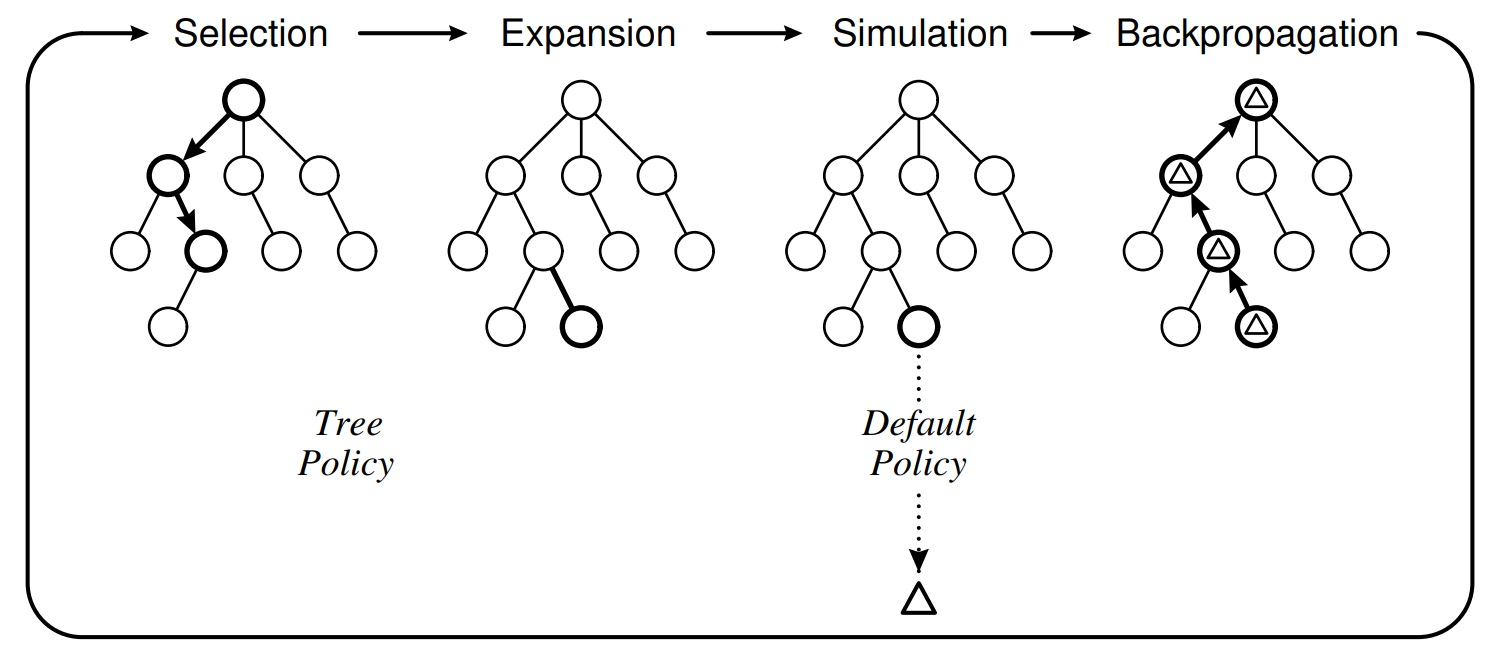
\includegraphics[width=\textwidth]{mcts-steps.jpg}
  \end{center}
  \caption{MCTS steps, credit to \cite{mcts-survey}}
  \label{fig:mcts-steps}
\end{figure}

\subsubsection{Selection}
Starting at the root node, select the child node by tree policy. Then recursively select child nodes through the tree until an ``expandable node'' is reached. A node is expandable if it represents a nonterminal state and has unvisited children (i.e. unexpanded).

\subsubsection{Expansion}
One (or more) child nodes are added to expand the tree, according to the available actions.

\subsubsection{Simulation (Rollout)}
A simulation is run from the new node(s) according to the default policy to produce an outcome.
\subsubsection{Backpropagation}
The simulation result is ``backed up'' (i.e. backpropagated) through the selected nodes to update their statistics.

\subsection{Exploration and exploitation}
Maintaining a balance between exploration and exploitation is an important part of implementing decision-making algorithms such as MCTS. During MCTS processes, all nodes have some chance of being randomly picked, which allows new decisions to be made so that new and better outcomes can be discovered. This is called exploration. At the same time, nodes that lead to a winning state will have a higher chance of being picked again in subsequent \glspl{playout}. This is called exploitation.

\subsection{UCB policy}
One of the most commonly used tree policies in MCTS is UCB (Upper Confidence Bound) \cite{RN2020}. As UCB is commonly used in \gls{multi-armed-bandit-problem}, the process in selection phase can be modelled accordingly. A child node j is selected to maximize:

\begin{equation}
  \label{eq:UCB}
  \mathrm{UCB} = \overline{X}_j + 2C_p\sqrt{\frac{2\ln n}{n_j}} 
\end{equation}

where $n$ is the number of times a parent node has visited, $n_j$ is the number of times a child node has visited, $X_j$ is the average reward of the parent node, and $C_p > 0$ is a constant.

In (\ref{eq:UCB}), the two terms are the exploitation term and the exploration term, respectively. If a node has been explored a few times, the exploration term will be high as a denominator $n_j$. $C_p$ is a constant that balances between exploitation and exploration.

\subsection{Winning action selection} \label{winning-action}
MCTS continues to run four steps until the endgame condition is met or the computation budget is reached. Then, the action of the root node is selected by some criteria. \newline Browne says that there are four criteria for selecting winning action, based on their survey \cite{mcts-survey}:

\begin{enumerate}
  \item \textbf{Max}: Select the action that gives the most rewards.
  \item \textbf{Robust}: Select the action that visited the most. 
  \item \textbf{Max-Robust}: Select the action that has the most rewards and visits. If none exist, continue searching until they are found.
  \item \textbf{Secure}: Select the action that maximizes the lower confidence bound.
\end{enumerate}

% TODO: add citations to MCTS wikipedia

\subsection{MCTS with imperfect information game and uncertainty}

In a deterministic game, MCTS can generate future states in nodes that will be found when performing an action. This is called a Closed Loop MCTS \cite{Perez_Liebana_2015}. But when nondeterministic actions come into concern, such as rolling dice or drawing random cards, we can still use a Closed Loop MCTS to generate all available possible outcomes as states and play out each one. However, it should be noted that this approach will make the game tree grows exponentially. 

An approximate solution is to use an Open Loop MCTS. Open Loop MCTS only stores the statistics in the nodes, not the states. Instead, the state at a node must be computed by playing actions along the path from the root node to the current node. This way, a node does not represent a state but a series of actions executed starting from the initial state of the game.

To handle imperfect information and uncertainty, a game can be converted into a determistic game using \textit{determinization}, the process of sampling all possible outcomes of all chance events, making it fully observable \cite{mcts-survey}. For example, rolling dice can be simulated with a predetermined sequence of dice rolls.

% \section{Reinforcement learning} % TODO: 
% \cite{Reinforcement-Learning} Reinforcement learning (RL) is a popular method used in many branches of applications, including game optimization, industry automation, telecommunications, etc. There are five main elements of reinforcement learning:

% \begin{enumerate}
%   \item Agent: the player who makes a decision about what action to take
%   \item Environment: the world in which an agent takes actions
%   \item State: current situation of the agent
%   \item Reward: feedback from the environment
%   \item Policy: how agents make decisions
% \end{enumerate}

% \tikzstyle{block} = [rectangle, rounded corners, 
% minimum width=3cm, 
% minimum height=1cm,
% text centered, 
% draw=black]

% \tikzstyle{small_block} = [rectangle, rounded corners, 
% minimum width=2cm, 
% minimum height=1cm,
% text centered, 
% draw=black]

% \tikzstyle{dashed_one_side} = [draw, rectangle, dashed, inner sep=2em]

% \tikzstyle{arrow} = [draw, thick, -latex']

% \begin{figure}
%   \centering
%   \begin{tikzpicture}[node distance=2cm]
%     \node (env) [block] {Environment};
%     \node (agent) [block, below of=env] {Agent};
%     \node (poli) [small_block, below of=agent] {Policy};
  
%     \begin{scope}
%       \draw [arrow] (env)-- ($(env.east)-(-0.5,0)$) |- node[anchor=center, right, pos=0.225] {State, Reward} (agent);
%       \draw [arrow] (agent)--($(agent.west)-(0.5,0)$) |- node[anchor=center, left, pos=0.275] {Action} (env);
%       \draw [arrow] (poli) -- (agent);
%       \draw [arrow] (agent) -- (poli);
%     \end{scope}
%   \end{tikzpicture}
  
%   \caption{Reinforcement Learning Model}
%   \label{fig:rl-flow}
% \end{figure}

% The concept of this method is to use agents to learn in a reward-punishment environment. The reinforcement learning model is described in figure \ref{fig:rl-flow}. The goal of reinforcement learning is to learn a policy that maximizes the reward the agent will receive. At first, the agent will be given the objective they must achieve. At each timestep of learning, the agent will receive the current state and available actions. Then, the agent will decide what actions to take from the policy they have, moving to a new state. By using the reward function, the feedback is returned to the agent to tell how well they behave or how they take actions. The agent will use that feedback to update their policy and then take another action, repeating the process until the agent has reached its objectives.

% Reinforcement learning is different from supervised learning in that there is no correct answer in reinforcement learning; instead, the reinforcement agent decides how to carry out the given task. In supervised learning, the training data includes the answer key, so the model is trained with that answer.
 
%%%%%%

% \section{Second section}
% Section 2 text.

% \subsection{Subsection heading goes here}

% Subsection 1 text

% \subsubsection{Subsubsection 1 heading goes here}
% Subsubsection 1 text

% \subsubsection{Subsubsection 2 heading goes here}
% Subsubsection 2 text

% \section{Third section}
% Section 3 text. The dielectric constant\index{dielectric constant}
% at the air-metal interface determines
% the resonance shift\index{resonance shift} as absorption or capture occurs
% is shown in Equation~\eqref{eq:dielectric}:

% \begin{equation}\label{eq:dielectric}
% k_1=\frac{\omega}{c({1/\varepsilon_m + 1/\varepsilon_i})^{1/2}}=k_2=\frac{\omega
% \sin(\theta)\varepsilon_\mathit{air}^{1/2}}{c}
% \end{equation}

% \noindent
% where $\omega$ is the frequency of the plasmon, $c$ is the speed of
% light, $\varepsilon_m$ is the dielectric constant of the metal,
% $\varepsilon_i$ is the dielectric constant of neighboring insulator,
% and $\varepsilon_\mathit{air}$ is the dielectric constant of air.

% \section{About using figures in your report}

% % define a command that produces some filler text, the lorem ipsum.
% \newcommand{\loremipsum}{
%   \textit{Lorem ipsum dolor sit amet, consectetur adipisicing elit, sed do
%   eiusmod tempor incididunt ut labore et dolore magna aliqua. Ut enim ad
%   minim veniam, quis nostrud exercitation ullamco laboris nisi ut
%   aliquip ex ea commodo consequat. Duis aute irure dolor in
%   reprehenderit in voluptate velit esse cillum dolore eu fugiat nulla
%   pariatur. Excepteur sint occaecat cupidatat non proident, sunt in
%   culpa qui officia deserunt mollit anim id est laborum.}\par}

% \begin{figure}
%   \centering

%   \fbox{
%      \parbox{.6\textwidth}{\loremipsum}
%   }

%   % To include an image in the figure, say myimage.pdf, you could use
%   % the following code. Look up the documentation for the package
%   % graphicx for more information.
%   % \includegraphics[width=\textwidth]{myimage}

%   \caption[Sample figure]{This figure is a sample containing \gls{lorem ipsum},
%   showing you how you can include figures and glossary in your report.
%   You can specify a shorter caption that will appear in the List of Figures.}
%   \label{fig:sample-figure}
% \end{figure}

% Using \verb.\label. and \verb.\ref. commands allows us to refer to
% figures easily. If we can refer to Figures
% \ref{fig:walrus} and \ref{fig:sample-figure} by name in the {\LaTeX}
% source code, then we will not need to update the code that refers to it
% even if the placement or ordering of the figures changes.

% \loremipsum\loremipsum

% % This code demonstrates how to get a landscape table or figure. It
% % uses the package lscape to turn everything but the page number into
% % landscape orientation. Everything should be included within an
% % \afterpage{ .... } to avoid causing a page break too early.
% \afterpage{
%   \begin{landscape}
%   \begin{table}
%     \caption{Sample landscape table}
%     \label{tab:sample-table}

%     \centering

%     \begin{tabular}{c||c|c}
%         Year & A & B \\
%         \hline\hline
%         1989 & 12 & 23 \\
%         1990 & 4 & 9 \\
%         1991 & 3 & 6 \\
%     \end{tabular}
%   \end{table}
%   \end{landscape}
% }

% \loremipsum\loremipsum\loremipsum

% \section{Overfull hbox}

% When the \verb.semifinal. option is passed to the \verb.cpecmu. document class,
% any line that is longer than the line width, i.e., an overfull hbox, will be
% highlighted with a black solid rule:
% \begin{center}
% \begin{minipage}{2em}
% juxtaposition
% \end{minipage}
% \end{center}

% \section{\ifenglish%
% \ifcpe CPE \else ISNE \fi knowledge used, applied, or integrated in this project
% \else%
% ความรู้ตามหลักสูตรซึ่งถูกนำมาใช้หรือบูรณาการในโครงงาน
% \fi
% }

% อธิบายถึงความรู้ และแนวทางการนำความรู้ต่างๆ ที่ได้เรียนตามหลักสูตร ซึ่งถูกนำมาใช้ในโครงงาน

% \section{\ifenglish%
% Extracurricular knowledge used, applied, or integrated in this project
% \else%
% ความรู้นอกหลักสูตรซึ่งถูกนำมาใช้หรือบูรณาการในโครงงาน
% \fi
% }

% อธิบายถึงความรู้ต่างๆ ที่เรียนรู้ด้วยตนเอง และแนวทางการนำความรู้เหล่านั้นมาใช้ในโครงงาน

\chapter{\ifproject%
\ifenglish Project Structure and Methodology\else โครงสร้างและขั้นตอนการทำงาน\fi
\else%
\ifenglish Project Structure\else โครงสร้างของโครงงาน\fi
\fi
}

The two main components of this project: \RootOurs{} and \RootAI.

% ในบทนี้จะกล่าวถึงหลักการ และการออกแบบระบบ

\makeatletter

% \renewcommand\section{\@startsection {section}{1}{\z@}%
%                                    {13.5ex \@plus -1ex \@minus -.2ex}%
%                                    {2.3ex \@plus.2ex}%
%                                    {\normalfont\large\bfseries}}

\makeatother
%\vspace{2ex}
% \titleformat{\section}{\normalfont\bfseries}{\thesection}{1em}{}
% \titlespacing*{\section}{0pt}{10ex}{0pt}

\section{\RootOurs}
\RootOurs{} is the game environment that mimics \RootV{} in a game of \Marquise{} versus \Eyrie. It has the following features:
\begin{itemize}
  \item Simulate the current state of the game
  \item Generate all possible actions (``legal actions'') for the current player at the current state of the game
  \item Change state according to the selected action 
  % \begin{itemize}
  %   \item With option for whether the simulation will randomize the non-deterministic actions by itself or whether the player can input a specific outcome value for the non-deterministic actions.
  % \end{itemize}
\end{itemize}


% From P Khem's 
% This module enables other services to communicate with the dictionary. It performs querying
% words and adding new words on the request. There is only a single dictionary management
% system per back-end service. The system performs word querying and word modifying in
% the database, which the back-end service cannot do directly.
\section{\RootAI}
\RootAI{} is the framework that allows humans and AI agents to interact with \RootOurs{} instance's environment.

There are 2 agent implementation methods: Random decision and Monte Carlo Tree Search (MCTS).

\subsection{Random decision}
The agent constructed using the random decision method will uniformly select an action from all legal actions at the current state. The list of legal actions has a \gls{discrete-uniform-distribution}, with each action having an equal likelihood of being chosen. % TODO: cite Wiki: discrete uniform distribution

% The agent built with random decision method will randomly select actions where all action has a uniform probability to be picked.

\subsection{Monte Carlo tree search (MCTS)} % TODO: add problem with current MCTS and Root
The agent will perform a tree search at the current state, determine which action has the highest probability of winning the game, and take that action. The winning probability of each action will be calculated using the MCTS approach.

% TODO: rework this sentence: "The winning probability of each action will be calculated using the MCTS approach."

\subsubsection{One-Depth MCTS}
``One-Depth MCTS'', similar to \textit{Flat Monte Carlo} \cite{mcts-survey}, is an MCTS agent that we implemented as a proof-of-concept for demonstrating that MCTS algorithm works with \RootB{}. It is called One-Depth because it only performs the legal action then immediately rollout from that state; not making any expansion down more than the first depth.

\subsubsection{General MCTS}
``General MCTS'' is the main MCTS algorithm in our project. We use a specific variant of MCTS called Open-Loop MCTS as a basis of implementation for this agent due to nondeterministic mechanism in this board game.

General MCTS has multiple parameters which can be customized to create multiple variants of MCTS. There are 6 parameters that we implemented, including: \texttt{reward-function}, \texttt{expand-count}, \texttt{rollout-no}, \texttt{time-limit}, \texttt{action-count-limit}, and \texttt{best-action-policy}.

\begin{enumerate}
  \item \textbf{\texttt{reward-function}}: The MCTS must determine how ``good'' the state at the end of a rollout is. This is done using the reward-function. There are 4 options for this parameter:
  \begin{itemize}
    \item \texttt{win}: considers whether the player wins; 1 if win, 0 otherwise
    \item \texttt{vp-difference}: considers the VP differences of the current player and the enemy player; \texttt{vp\_player} - \texttt{vp\_enemy}
    \item \texttt{vp-difference-bin}: considers the VP differences; 1 if > 0,  0 otherwise
    \item \texttt{vp-difference-relu}: considers the VP differences is \texttt{d}; \texttt{d} if \texttt{d} > 0, 0 otherwise  
  \end{itemize}
  \item \textbf{\texttt{expand-count}}: Whenever the MCTS expands the game tree, a node is added to the tree. This parameter limits the number of expansion. We could expand indefinitely until the entire tree is searched, which should result in a better outcome, but that would take too much computation time. That is the reason that this parameter exists.
  \item \textbf{\texttt{rollout-no}}: Whenever the MCTS expands, it must perform a number rollouts to determine the reward of that node. This parameter controls the amount of rollouts per node. A rollout is bound to come across some nondeterministic actions which could result in varying outcome of that rollout. Multiple rollouts per node can be used to help mitigate the varying outcomes.
  \item \textbf{\texttt{time-limit}}: A rollout may encounter an infinite loop or may take a very long time. This parameter controls the time limit for each rollout. A rollout will immediately stop at its current state if a time limit is exceeded. % Note that from our experience, a rollout is pretty fast.
  \item \textbf{\texttt{action-count-limit}}: A rollout does not necessarily need to reach a game-ending state to stop. This parameter controls how many actions will be executed before stopping a rollout, i.e., how deep into the future will a rollout look.
  \item \textbf{\texttt{best-action-policy}}: As described in Section \ref{winning-action}, when the MCTS algorithm finishes, it must choose which legal action is the best. This parameter controls how the ``best'' legal action is picked. There are 3 options for this parameter:
  \begin{itemize}
    \item \texttt{max}: picks the legal action with the highest reward
    \item \texttt{robust}: picks the most visited legal action
    \item \texttt{secure}: picks the legal action that maximises the lower confidence bound
  \end{itemize}
\end{enumerate}

% TODO: add citations to UCB, secure

% \subsection{Reinforcement learning neural network (RLNN)}
% The agent constructed using RLNN will use RNN type model, taking the current state, past states, and past actions as input and outputing the probability of choosing each action from all legal actions in the current state. Then calculate the reward of that action using the reward function, which is yet to be defined. Adjust the neural network according to the reward, and adjust the agent’s current state to the new state in the feedback. % unconfirmed


% \begin{enumerate}
%   \item Agent: the player that's playing as \Marquise{} faction or \Eyrie{} faction
%   \item Environment: the map, opponent's state and action, draw pile, etc. in \RootOurs % not sure
%   \item State: all game components that belonged to the player
%   \item Reward: victory points earned, getting a win, or taking hold of clearing with matching suit to the played dominance card, all combined together through the reward function 
%   \item Policy: the neural network
% \end{enumerate}

% TODO: add evaluation method
% \chapter{\ifproject%
% \ifenglish Experimentation and Results\else การทดลองและผลลัพธ์\fi
% \else%
% \ifenglish System Evaluation\else การประเมินระบบ\fi
% \fi}
\chapter{
    \ifenglish Experimentation and Results\else การทดลองและผลลัพธ์\fi
}

\definecolor{eyrie}{HTML}{1E90FF}
\definecolor{marquise}{HTML}{FF6400}

% ในบทนี้จะทดสอบเกี่ยวกับการทำงานในฟังก์ชันหลักๆ

\section{Experimental Setup}

\subsection{Introductory experiment}
For introductory experiment, we will use random decision agent as it has the most basic implementation. Since we have not implemented \RootAI, we will conduct experiments by simulating \RootOurs \ with random actions option turned on, and collect the results. 

We will run 1000 \glspl{playout} using a random decision agent as each faction and collect the following statistics:
\begin{itemize}
    \item winning faction: \Marquise{} / \Eyrie
    \item winning condition: 30 victory points (vp) / dominance card (dominance)
    \item number of turns played (the number of birdsong phase played)
    \item whose turn was it when the game ends: \Marquise{} / \Eyrie
    \item victory points of \Marquise{} when the game ends
    \item victory points of \Eyrie{} when the game ends
    \item dominance card of the winning faction: none / bird / fox / rabbit / mouse
\end{itemize}

\section{Results}

\subsection{Introductory experiment's results}

\begin{figure}
    \centering
    \begin{tikzpicture}
        \begin{axis}[
            width  = 0.5*\textwidth,
            height = 8cm,
            major x tick style = transparent,
            ybar=2*\pgflinewidth,
            bar width=24pt,
            ymajorgrids = true,
            ylabel = {Number of Wins},
            symbolic x coords={Dominance Card,Victory Point},
            xtick = data,
            enlarge x limits=0.5,
            enlarge y limits=0.1,
            ymax = 1000,
            legend cell align=left,
            legend style={
                at={(0.5,-0.15)},
                anchor=north,
                legend columns=-1
            },
            nodes near coords,
        ]
            \addplot[style={eyrie,fill=eyrie,mark=none}]
                coordinates {(Dominance Card, 230) (Victory Point,44)};
    
            \addplot[style={marquise,fill=marquise,mark=none}]
                 coordinates {(Dominance Card,695) (Victory Point,31)};
    
            \legend{\Eyrie, \Marquise}
        \end{axis}
    \end{tikzpicture}
    \caption{The number of wins grouped by winning condition}
    \label{fig:wins-by-winner-condition}
\end{figure}

\subsubsection{High dominance card wins} \label{high-dominance-card-wins}
Dominance card wins happen way more often than victory points wins as seen in figure \ref{fig:wins-by-winner-condition}. Our speculation is that it is the action generation in \RootOurs \ that makes the ``Activate Dominance Card'' action have a higher likelihood of being picked. \RootOurs generates actions in a manner that is more suitable for human players, e.g., in the move action, the agent needs to select a start clearing, then a destination clearing, and then how many warriors to move. These are done as three separate actions, while in reality, the action of ``Move X warriors from A to B'' should be counted as one action.

\subsubsection{\Marquise's high dominance card wins}
\Marquise \ have a higher chance to win with dominance card (figure \ref{fig:wins-by-winner-condition}). Our speculation is that because at the start of the round, \Marquise \ have control over clearings except the one that \Eyrie \ starts in, therefore, if \Eyrie does not play properly to take control of the clearings, \Marquise will likely win upon the activation of a dominance card of any suit.

\subsubsection{\Eyrie's high victory points wins}
\Eyrie \ have a higher chance to win with victory points (figure \ref{fig:wins-by-winner-condition}). Although there are not many data for rounds with victory points wins, our experience during development where we turned of the dominance card mechanics also have more \Eyrie \ victory points win. Our speculation is that this is due to \Eyrie's passive earning of victory points, all they need to do is protect their roosts and don't turmoil too much. In contrast, \Marquise \ needs to actively build buildings to earn points, which from the issue about action generation in \ref{high-dominance-card-wins}, action of building buildings might not have the correct likelihood of being picked.



% TODO: add result graph
\ifproject
\chapter{\ifenglish Conclusions and Discussions\else บทสรุปและข้อเสนอแนะ\fi}

\section{\ifenglish Conclusions\else สรุปผล\fi}

An online forum discussion (and our personal experiences) stated that, a normal game of Root lasts 7-10 rounds. For a 2 players scenario, this is around 14-20 turns. Comparing that to our best performing MCTS AI agents which have 15.389 and 13.681 average turns to end (average match length), \Marquise{} and \Eyrie{}, respectively. We have concluded that our MCTS AI agents are able to intelligently play \RootB{}.

The best MCTS variant for \Marquise{} is from config number 85. It achieved average win rate against top 5 \Eyrie{} agents of 56.0\%. It has the following parameters:
\begin{itemize}
    \item \textbf{\texttt{reward-function}}: \texttt{vp-difference}
    \item \textbf{\texttt{expand-count}}: 200
    \item \textbf{\texttt{rollout-no}}: 1
    \item \textbf{\texttt{time-limit}}: -1 (no-limit)
    \item \textbf{\texttt{action-count-limit}}: 100
    \item \textbf{\texttt{best-action-policy}}: \texttt{max}
\end{itemize}
The best MCTS variant for \Eyrie{} is from config number 184. It achieved average win rate against top 5 \Marquise{} agents of 63.4\%. It has the following parameters:
\begin{itemize}
    \item \textbf{\texttt{reward-function}}: \texttt{vp-difference}
    \item \textbf{\texttt{expand-count}}: 200
    \item \textbf{\texttt{rollout-no}}: 1
    \item \textbf{\texttt{time-limit}}: -1 (no-limit)
    \item \textbf{\texttt{action-count-limit}}: 20
    \item \textbf{\texttt{best-action-policy}}: \texttt{robust}
\end{itemize}

\section{\ifenglish Challenges\else ปัญหาที่พบและแนวทางการแก้ไข\fi}

\begin{itemize}
    \item We understimated the complexity of \RootB{}. We estimated to complete the core implementation of \RootOurs{} within 3 weeks but it has taken us 3 months. We should give more consideration to carefully estimating the size of the tasks so that we can better plan out the project.
    \item For the MCTS algorithm to be intelligent, it must be able to look deep into multiple possibilities. To achieve this level of intelligence in an acceptable amount of time requires a high amount of processing power. The department's server, which has a lot of CPU cores, along with us reducing the number of variants to half, helped us achieve that. Otherwise, we wouldn't have been able to simulate as many battles as we did. This is another lesson in planning for a project that requires processing power; you need a lot of processing power if you don't want to spend a lot of time.
    \item This project is more of a research-style than a software-development project. We have never done a project in this manner before and this is our first time doing it like this. We gained lots of experience from this.
\end{itemize}

\section{\ifenglish%
Suggestions and further improvements
\else%
ข้อเสนอแนะและแนวทางการพัฒนาต่อ
\fi
}

\begin{itemize}
    \item To connect \RootAI{} to an instance of \RootV{} and have the AIs play against each other will be the ultimate testing method of whether our AI is better than \RootV{}'s AI. 
    \item AIs for \RootB{} can be implemented using other methods such as reinforcement learning, artificial neural networks, etc.
    \item If the user interface is made with something else such as a game engine, human players would be able to play \RootOurs{} more easily then the current method of arrow keys and spacebar. Though doing that would require more time actually developing it and connecting to the logic code.
    \item This project does not need to be written in Python. It was written in Python because our original scope includes reinforcement learning with neural network, which we planned to use PyTorch and/or Tensorflow in those parts.
\end{itemize}

% This project is about creating an AI to play an asymmetrical game using reinforcement learning techniques. This project expands the capabilities of AI from traning against itself to training against an opponent whose doesn't play the same rule as it. In the future, this can

\fi

\bibliography{report}

\ifproject
\normalspacing
\appendix
\chapter{Appendix}

% Text for the first appendix goes here.

\section{Project resources}

The resources associated to this project can be accessed via the following links:
\begin{itemize}
    \item \textbf{RootAI source code:} \url{https://github.com/iambaangkok/RootAI}
    \item \textbf{Video explanation:} \url{https://youtu.be/p06QnM63f4o}
    \item \textbf{RootAI 261492 final report:} \url{https://github.com/DarkTXYZ/RootAI-492-Final-Report}
    \item \textbf{RootAI 261491 final report:} \url{https://github.com/iambaangkok/RootAI-491-Final-Report}
\end{itemize}

% Text for a section in the first appendix goes here.

% test ทดสอบฟอนต์ serif ภาษาไทย

% \textsf{test ทดสอบฟอนต์ sans serif ภาษาไทย}

% \verb+test ทดสอบฟอนต์ teletype ภาษาไทย+

% \texttt{test ทดสอบฟอนต์ teletype ภาษาไทย}

% \textbf{ตัวหนา serif ภาษาไทย \textsf{sans serif ภาษาไทย} \texttt{teletype ภาษาไทย}}

% \textit{ตัวเอียง serif ภาษาไทย \textsf{sans serif ภาษาไทย} \texttt{teletype ภาษาไทย}}

% \textbf{\textit{ตัวหนาเอียง serif ภาษาไทย \textsf{sans serif ภาษาไทย} \texttt{teletype ภาษาไทย}}}

% \chapter{\ifenglish Manual\else คู่มือการใช้งานระบบ\fi}

% Manual goes here.


%% Display glossary (optional) -- need glossary option.
\ifglossary\glossarypage\fi

%% Display index (optional) -- need idx option.
\ifindex\indexpage\fi

\begin{biosketch}
\begin{center}
  \includegraphics[width=1.5in]{mugshot.jpg}
\end{center}
Your biosketch goes here. Make sure it sits inside
the \texttt{biosketch} environment.
\end{biosketch}
\fi % \ifproject
\end{document}
